\documentclass[a4paper, 12pt]{article}
\usepackage[slovene]{babel}
\usepackage[utf8]{inputenc}
\usepackage{amsmath}
\usepackage{amssymb}
\usepackage{listings}
\usepackage{hyperref}
\usepackage{tikz}
\usetikzlibrary{positioning}
\usetikzlibrary{arrows}

\begin{document}
\title{Population dynamics in a food chain}
\author{Domen Mohorčič, Larsen Cundrič, Mustafa Grabus}
\maketitle

\section{Problem}
Modelirali bomo dinamiko populacij različnih vrst, odnosi med vrstami pa so predstavljeni
na naslednji sliki: \\
\begin{center}
	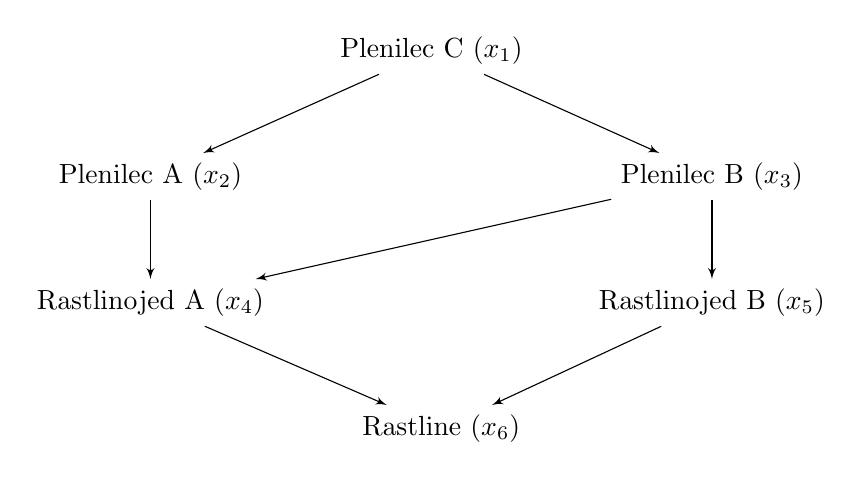
\begin{tikzpicture}
		\tikzset{edge/.style = {->,> = latex'}}
		\node (A) {Plenilec C ($ x_{1} $)};
		\node[below left=of A] (B) {Plenilec A ($ x_{2} $)};
		\node[below right=of A] (C) {Plenilec B ($ x_{3} $)};
		\node[below=of B] (D) {Rastlinojed A ($ x_{4} $)};
		\node[below=of C] (E) {Rastlinojed B ($ x_{5} $)};
		\node[below right=of D] (F) {Rastline ($ x_{6} $)};
		\draw[edge] (A) edge (B) edge (C);
		\draw[edge] (B) edge (D);
		\draw[edge] (C) edge (D) edge (E);
		\draw[edge] (D) edge (F);
		\draw[edge] (E) edge (F);
	\end{tikzpicture}
\end{center}
Puščice označujejo smer prehranjevanja (npr. Plenilec A se prehranjuje z Rastlinojedom A).
Z $ x_{i} $ označimo velikost posamezne populacije. Sprememba velikosti posamezne populacije
je tako odvisna od naravnega prirastka/smrtnosti, smrtnosti zaradi ulova in prirastka zaradi
prehranjevanja. Ulov in prehranjevanje sta odvisna od velikosti ustreznih drugih populacij,
naravni prirastek/smrtnost pa je odvisna samo od velikosti populacije. Dinamiko $ i $-te
populacije lahko opišemo tako:
\begin{equation}
	\dot x_{i} = x_{i}\cdot b_{i} + \sum_{i \not = j} a_{ij}\cdot x_{i}\cdot x_{j}
\end{equation}
kjer je $ x_{i} $ velikost $ i $-te populacije, $ b_{i} $ je koeficient naravnega prirastka/smrtnosti,
$ a_{ij}\cdot x_{i}\cdot x_{j} $ pa je sprememba $ i $-te populacije glede na interakcijo z $ j $-to populacijo.

\section{Reševanje}

\subsection{Naloga 1}
Sistem diferencialnih enačb za naš primer je naslednji:
\begin{align*}
	&\dot x_{1} = x_{1}\cdot(b_{1}+a_{12}\cdot x_{2}+a_{13}\cdot x_{3}) \\
	&\dot x_{2} = x_{2}\cdot(b_{2}+a_{21}\cdot x_{1}+a_{24}\cdot x_{4}) \\
	&\dot x_{3} = x_{3}\cdot(b_{3}+a_{31}\cdot x_{1}+a_{34}\cdot x_{4}+a_{35}\cdot x_{5}) \\
	&\dot x_{4} = x_{4}\cdot(b_{4}+a_{42}\cdot x_{2}+a_{43}\cdot x_{3}+a_{46}\cdot x_{6}) \\
	&\dot x_{5} = x_{5}\cdot(b_{5}+a_{53}\cdot x_{3}+a_{56}\cdot x_{6}) \\
	&\dot x_{6} = x_{6}\cdot(b_{6}+a_{64}\cdot x_{4}+a_{65}\cdot x_{5}) \\
\end{align*}
$ x_{i} $ predstavlja velikost i-te populacije, $ \dot x_{i} $ pa predstavlja spremembo
i-te populacije v odvisnosti od velikosti ostalih populacij. Velikosti posameznih vrst
bomo zapisali v vektor $ X = \left[x_{1}, x_{2}, x_{3}, x_{4}, x_{5}, x_{6}\right]^{T} $.
Sistem diferencialnih enačb pa bomo zapisali v vektor $ \dot X $:
\begin{equation}
	\dot X =
	\begin{bmatrix}
		\dot x_{1} \\
		\dot x_{2} \\
		\dot x_{3} \\
		\dot x_{4} \\
		\dot x_{5} \\
		\dot x_{6} \\
	\end{bmatrix}
	=
	\begin{bmatrix}
		x_{1}\cdot(b_{1}+a_{12}\cdot x_{2}+a_{13}\cdot x_{3}) \\
		x_{2}\cdot(b_{2}+a_{21}\cdot x_{1}+a_{24}\cdot x_{4}) \\
		x_{3}\cdot(b_{3}+a_{31}\cdot x_{1}+a_{34}\cdot x_{4}+a_{35}\cdot x_{5}) \\
		x_{4}\cdot(b_{4}+a_{42}\cdot x_{2}+a_{43}\cdot x_{3}+a_{46}\cdot x_{6}) \\
		x_{5}\cdot(b_{5}+a_{53}\cdot x_{3}+a_{56}\cdot x_{6}) \\
		x_{6}\cdot(b_{6}+a_{64}\cdot x_{4}+a_{65}\cdot x_{5}) \\
	\end{bmatrix}
\end{equation}
V vektorju $ b = \left[b_{1}, b_{2}, b_{3}, b_{4}, b_{5}, b_{6}\right]^{T} $ so koeficienti naravnega prirastka/smrtnosti,
ki je za rastline ($ x_{6} $) pozitiven, za vse ostale pa negativen. \\
Sistem enačb za dani primer lahko tako zapišemo kot
\begin{equation}
	\dot X = X*(b+A\cdot X)
\end{equation}
($ * $ predstavlja množenje po elementih),
kjer matrika $ A $ vsebuje koeficiente hranjenja in plenjenja $ a_{ij} $:
\begin{equation}
	A =
	\begin{bmatrix}
		0 & a_{12} & a_{13} & 0 & 0 & 0 \\
		a_{21} & 0 & 0 & a_{24} & 0 & 0 \\
		a_{31} & 0 & 0 & a_{34} & a_{35} & 0 \\
		0 & a_{42} & a_{43} & 0 & 0 & a_{46} \\
		0 & 0 & a_{53} & 0 & 0 & a_{56} \\
		0 & 0 & 0 & a_{64} & a_{65} & 0 \\
	\end{bmatrix}
\end{equation}
Koeficient $ a_{ij} $ predstavlja interakcijo vrste $ i $ in $ j $. Pozitivna vrednost pomeni, da se vrsta
$ i $ prehranjuje z vrsto $ j $, negativna pa ravno nasprotno. Vrsta s sabo nima take interakcije, zato
so elemeniti $ a_{i=j} = 0 $. Koeficienta $ a_{ij} $ in $ a_{ji} $ nista nujno nasprotna, saj lahko plenilska
vrsta poje več plena, kot pa ima koristi od tega. \\
Za začetek smo določili $ b = \left[-0.1, -0.1, -0.1, -0.05, -0.05, 0.3\right]^{T} $
in 
\begin{equation}
	A = 
	\begin{bmatrix}
		0 & 0.5 & 0.7 & 0 & 0 & 0 \\
		-2 & 0 & 0 & 1 & 0 & 0 \\
		-8 & 0 & 0 & 1 & 4 & 0 \\
		0 & -6 & -1 & 0 & 0 & 2 \\
		0 & 0 & -1 & 0 & 0 & 1 \\
		0 & 0 & 0 & -2 & -5 & 0 \\
	\end{bmatrix}\cdot 0.001
\end{equation}

\subsection{Naloga 2}
Stacionarna rešitev sistema je, ko je vektor $ \dot X $ enak  $ 0 $. To pomeni, da je
$ X*(b+A\cdot X) = 0 $. Vektor $ X = 0 $ že zadosti našemu pogoju, vendar iščemo neničelno
rešitev. Za naša $ A $ in $ b $ je to $ X = \left[8.7, 28.7, 122.3, 117.4, 13.0, 172.3\right]^{T} $.
Slika rešitve po 100 iteracijah izgleda tako:\\
\begin{center}
	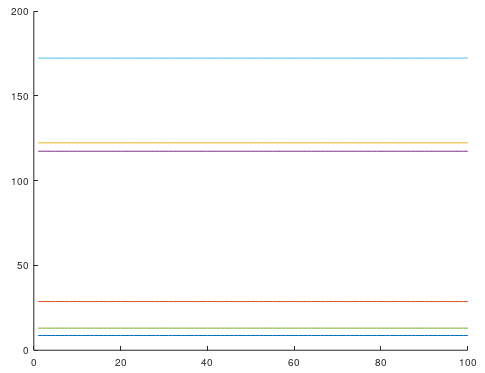
\includegraphics{stationary.png}
\end{center}

\subsection{Naloga 3}
Napisali smo funcijo {\sf simulatePopulation.m}, ki za vhod vzame matriko $ A $, vektor $ b $ in začetne
velikosti populacij v vektorju $ X $.
\begin{lstlisting}[language=Octave]
function retval = simulatePopulation (x0, b, A, n, fig)
    F = @(X, b, A) X.*(b+A*X);%enacba prirastka za vsako vrsto
    h = 0.1;%dolzina koraka

    tocke = zeros(6, n);
    x = x0;

    %%Simulacija
    for i = (1:n)
        x = x + rk4Step(F, x, h, b, A);
        tocke(:, i) = x;
    end

    figure(fig)
    hold on
    for i = (1:6)
        vektor = zeros(1, n);
        vektor(1, :) = tocke(i, :);
        plot(vektor);
    endfor

    lastX = x  
endfunction
  
%%Korak rk4
function val = rk4Step(f, x0, h, b, A)
    k1=feval(f, x0, b, A);
    k2=feval(f, x0 + k1*h/2, b, A);
    k3=feval(f, x0 + k2*h/2, b, A);
    k4=feval(f, x0 + k3*h, b, A);
    val = h*(k1+2*k2+2*k3+k4)/6;
endfunction
\end{lstlisting}

\subsection{Naloga 4}
Naredili smo simulacijo za začetne pogoje, ki se malo razlikujejo od $ X $. Dobili smo
$ X_{nov} = \left[9.0, 32.6, 125.9, 121.0, 16.5, 175.4\right]^{T} $, slika simulacije po 5000 iteracijah
pa izleda tako:\\
\begin{center}
	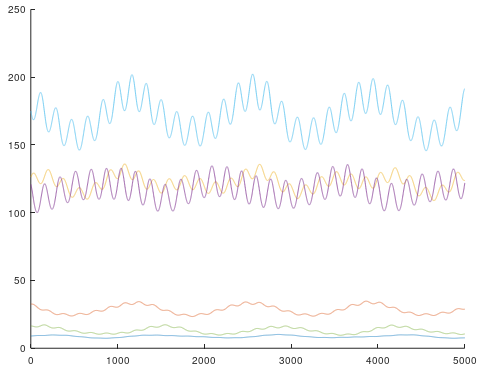
\includegraphics{stationary_almost.png}
\end{center}

\subsection{Naloga 5}
Preučili smo obnašanje sistema za različne vrednosti koeficientov in začetnih pogojev in našli
ciklično, asimptotično ciklično obnašanje in kaos.\\
Asimptotično ciklično obnašanje smo dobili z naslednjimi začetnimi vrednostmi:\\
$ A =
\begin{bmatrix}
	0 & 0.0041790 & 0.0014199 & 0 & 0 & 0 \\
	-0.0010902 & 0 & 0 & 0.0038366 & 0 & 0 \\
	-0.0019610 & 0 & 0 & 0.0031243 & 0.0038874 & 0 \\
	0 & -0.0022909 & 0.0029800 & 0 & 0 & 0.0053580 \\
	0 & 0 & -0.0032865 & 0 & 0 & 0.0059388 \\
	0 & 0 & 0 & -0.0028531 & -0.0031236 & 0 \\
\end{bmatrix} $, 
$ b =
\begin{bmatrix}
	-0.0824046 \\
	-0.0059820 \\
	-0.0192474 \\
	-0.0311698 \\
	-0.0448382 \\
	0.0549130 \\
\end{bmatrix} $ in
$ X =
\begin{bmatrix}
	23.2438 \\
	17.8982 \\
	5.2910 \\
	8.1907 \\
	10.0353 \\
	10.4537 \\
\end{bmatrix} $. \\
Vektor $ X $ se od stacionarne rešitve sistema razlikuje samo za $ 0.11196 $. Slika simulacije
sistema s takimi podatki pa je naslednja:
\begin{center}
	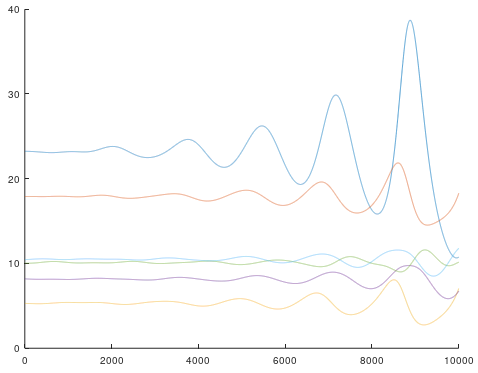
\includegraphics{asimptotic_cyclic.png}
\end{center}

Kaos pa smo dobili z naslednjimi koeficienti:\\
$ A =
\begin{bmatrix}
	0 & 0.0005993 & 0.0018995 & 0 & 0 & 0 \\
	-0.0010021 & 0 & 0 & 0.0007798 & 0 & 0 \\
	-0.0016327 & 0 & 0 & 0.0003364 & 0.0002603 & 0 \\
	0 & -0.0001513 & 0.0008657 & 0 & 0 & 0.0007994 \\
	0 & 0 & -0.0024918 & 0 & 0 & 0.0025529 \\
	0 & 0 & 0 & -0.0009197 & -0.0003923 & 0 \\
\end{bmatrix} $, 
$ b =
\begin{bmatrix}
	-0.0394982 \\
	-0.0159140 \\
	-0.0042202 \\
	-0.0326592 \\
	-0.0235321 \\
	0.0275829 \\
\end{bmatrix} $ in
$ X =
\begin{bmatrix}
	3.4576 \\
	13.4956 \\
	14.4207 \\
	25.7688 \\
	9.5432 \\
	21.9396 \\
\end{bmatrix} $. \\
Vektor $ X $ se od stacionarne rešitve razlikuje za $ 4.1805 $,
za sistem pa po 10000 iteracijah dobimo naslednjo naslednjo sliko:\\
\begin{center}
	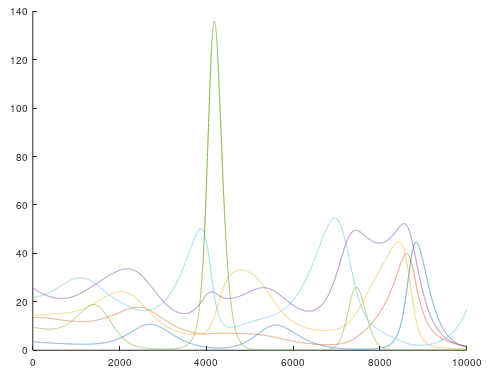
\includegraphics{caos.png}
\end{center}
Ciklično obnašanje smo opisali v poglavju Naloga 4.\\
Obnašanje sistema pa je odvisno od lastnih vrednosti jakobijeve matrike sistema
v stacionarni točki. Lastne vrednosti so kompleksne, od njihovega realnega dela pa
je odvisno obnašanje sistema. Če je realni del manjši od nič, je stacionarna točka
spiralni liak, če pa je pozitivna, je spiralni izvor.

\end{document}